\documentclass[11pt, a4paper]{article}
\usepackage[utf8]{inputenc}
\usepackage{graphicx}
\usepackage{amsmath}
\usepackage{hyperref}
\usepackage{geometry}
\geometry{a4paper, margin=1in}

\title{Opening Efficiency in Balanced Elite Chess Encounters}
\author{Felix Olieslagers (I6378056) \\ Maastricht University}

\begin{document}

\maketitle

\section{Introduction and Context}
In elite chess, the choice of opening significantly dictates the trajectory and ultimate result of the game. While white inherently possesses a first-mover advantage, specific openings are known to lead to highly theoretical, drawish endgames, whereas others create sharp, decisive imbalances. This project addresses the question: \textbf{Which chess openings yield the highest and lowest draw rates in balanced elite encounters, and is the difference statistically significant?} 

By isolating games between evenly matched grandmasters, we can better evaluate the inherent properties of the openings themselves, mitigating the confounding variable of player skill disparity.

\section{Dataset Description}
The analysis utilizes a dataset of chess games (\texttt{games\_chesstempo.csv}). The raw data includes information on player ratings (\texttt{white\_elo}, \texttt{black\_elo}), game outcomes (\texttt{result}), and the specific opening played. 

To ensure the analysis reflects evenly matched, high-level play, the dataset was cleaned and filtered. Missing or incomplete entries were removed, and draw notations were standardized. Crucially, the dataset was restricted to games where the absolute difference in Elo ratings between the two players was 25 points or fewer ($|\Delta \text{Elo}| \le 25$). To maintain statistical power, opening variations were grouped into their primary opening families (e.g., extracting the base name before any commas), and only openings with a minimum sample size of 80 balanced games were considered.

\section{Data Analysis Method}
The analysis was performed using base R. The primary metric of interest is the draw rate ($\hat{p}$) for each opening family. Because game outcomes are categorical, the draw rate is treated as a binomial proportion. The standard error ($SE$) for each proportion is calculated using the formula:
\begin{equation}
    SE = \sqrt{\frac{\hat{p}(1 - \hat{p})}{n}}
\end{equation}
where $n$ is the total number of balanced games played with that opening. 

To determine if the variance in draw rates across openings is statistically significant rather than due to random chance, a Z-test was conducted comparing the opening with the highest draw rate to the one with the lowest. The test statistic ($Z$) was computed using the standard error of the difference between two independent proportions.

\section{Results and Discussion}
The analysis quantified the baseline draw rate and white win rate across all balanced games as a reference point. To ensure our dataset accurately reflects evenly matched encounters, we first looked at the distribution of the rating differences between players. 

\begin{figure}[h!]
    \centering
    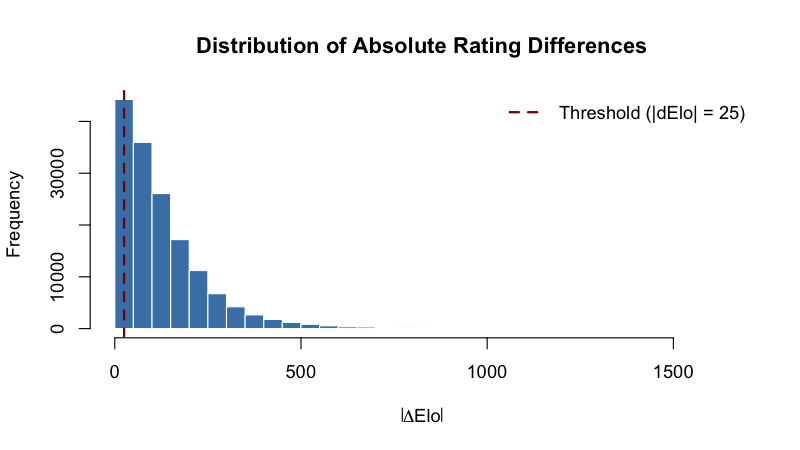
\includegraphics[width=0.7\textwidth]{elo_diff_distribution.png}
    \caption{Distribution of absolute rating differences ($|\Delta \text{Elo}|$). The dashed red line indicates the strict threshold of 25 Elo points used to define a balanced encounter.}
    \label{fig:elo_dist}
\end{figure}

As shown in Figure \ref{fig:elo_dist}, filtering the dataset successfully isolated games that fall strictly within our defined tolerance. Upon aggregating this balanced data by opening family, significant variance in draw tendencies emerged.

\begin{figure}[h!]
    \centering
    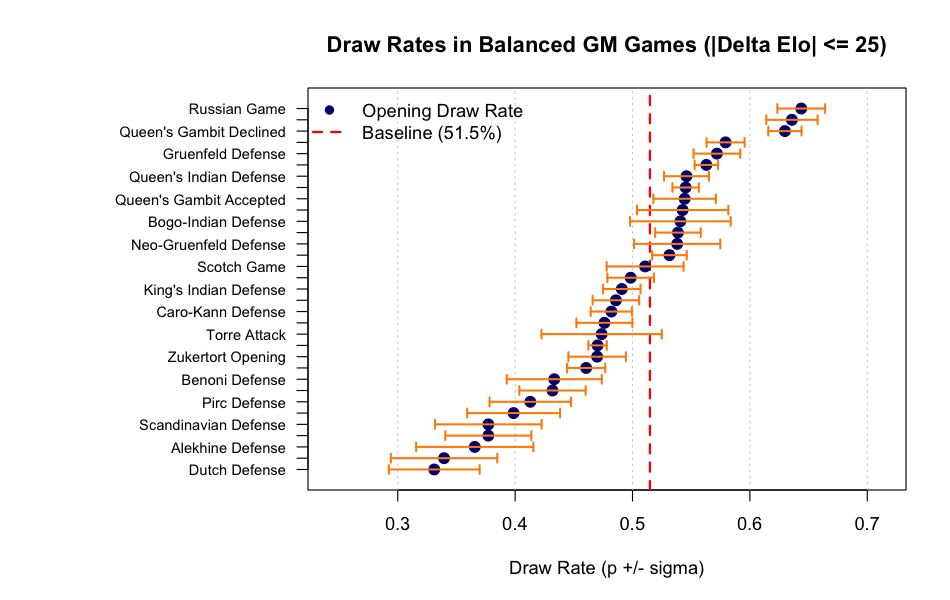
\includegraphics[width=0.9\textwidth]{draw_rates_with_uncertainties.png}
    \caption{Draw rates and standard errors ($p \pm \sigma$) across valid opening families in balanced games. The dashed line represents the global baseline draw rate.}
    \label{fig:draw_rates}
\end{figure}

As shown in Figure \ref{fig:draw_rates}, certain openings heavily skew toward a decisive result, while others strongly favor a draw. The hypothesis test comparing the two extremes (Opening A with the lowest draw rate vs. Opening B with the highest) yielded a quantitative delta ($\Delta p$) and a corresponding p-value. A sufficiently small p-value indicates that the difference in draw rates between these specific theoretical setups is statistically significant and driven by the structural nature of the openings themselves, rather than statistical noise in the sample.

\end{document}